\chapter{Introdução}
\label{Cap:Introducao}

Escassez de recursos, baixa remuneração, custos crescentes, disponibilidade de recursos hídricos e o desperdício fazem com que a economia de energia elétrica no Brasil seja vista como uma necessidade para os moradores de cidades \cite{eflul}. Grande parte do consumo mensal de energia elétrica é manifestada através do uso de eletrodomésticos. Portanto são comuns as ideias de compra ou troca de equipamentos por outros mais eficientes quanto ao consumo de energia, ou mudanças nos hábitos de uso destes nas residências. Entretanto, surgem dúvidas: ``Qual equipamento devo trocar? Por que o valor da conta de luz veio alta mesmo tendo desligado todos os equipamentos antes de viajar? Será que eu deixei o ferro de passar ligado em casa?'' Muitas vezes os moradores de residência não têm as informações necessárias para tomar decisões seguras e proativas ou as informações não estão disponíveis em um formato compreensível. 

Há ferramentas existentes que podem ajudar a população na área de controle de consumo de energia elétrica como OpenEnergyMonitor \cite{open_energy_monitor} e Neurio \cite{neurio_site}. Ambas possuem dispositivos para serem instalados diretamente no quadro elétrico, e no caso da Neurio, é possível estimar o consumo por equipamento doméstico. Porém, como garantir que o consumo é de fato daquele equipamento em específico, e não apenas um ruído vindo de outro equipamento? O objetivo do projeto é o desenvolvimento de um sistema de monitoramento de consumo de energia em uma residência. No sistema há dispositivos de medição de consumo por equipamento, ou seja, o usuário não precisa manusear o quadro elétrico, basta conectar os dispositivos medidores aos equipamentos desejados. E além disso, esses dispositivos são interligados por uma rede sem fio, para garantir flexibilidade, facilidade de instalação e robustez, provendo conforto para o ambiente residencial.

Tendo os dados de consumo ao alcance do usuário também não é suficiente, é necessário mostrar transparência no perfil de consumo de seus equipamentos. Para isso, o projeto inclui o desenvolvimento de uma aplicação Web, onde é possível mostrar o consumo através de gráficos, além de outras funcionalidades como conversão de consumo de energia para unidades monetárias e traçar metas de consumo. Essas funcionalidades são alcançáveis remotamente através de serviços em nuvem utilizados, pertencentes à empresa Heroku. Através de dispositivos portáteis que o usuário tenha em mãos como smartphones, tablets e notebooks, este pode utilizar a aplicação Web em qualquer lugar com acesso à internet. 

O desenvolvimento do projeto é descrito neste trabalho, sempre dando preferência para o uso de hardware e software open-source, framework e linguagens de programação gratuitos. Para verificar o funcionamento do sistema, um protótipo do sistema é construído e os resultados estão descritos no trabalho.

\section{Objetivo}
\label{Sec:objetivo}

O trabalho descreve o desenvolvimento de um sistema para monitorar o uso de energia elétrica dentro de residência. O sistema consiste de dispositivos interligados por uma rede sem fio, para a coleta de medidas de consumo por equipamento e uma aplicação em nuvem, que apresenta as medidas coletadas através de uma interface simples e intuitiva. Além disso é construído um protótipo para cada componente do sistema.

\section{Motivação}
\label{Sec:motivacao}

Em 2015, devido à escassez de chuvas, houve uma queda significativa no nível dos reservatórios das principais hidrelétricas do Brasil e o uso mais intenso de termelétricas. Isso provocou reajustes altos, encarecendo a energia elétrica no país e o custo foi repassado para os consumidores finais, como se pode verificar nos jornais: G1 \cite{news_g1} e O Estado de S. Paulo \cite{news_secretaria_de_energia}.

Segundo relatório da COPAM/EPE \cite{copam_epe}, o consumo de energia elétrica pela região Sudeste corresponde a 51,73\% da matriz energética do Brasil, ou seja, é a região geográfica que gasta mais energia elétrica. Analisando o estado de São Paulo, o município com maior participação no consumo estadual de energia elétrica é São Paulo, consumindo 39,90\% do estado \cite{itu}. Além disso, notícia da Folha \cite{folha} revela que de toda energia consumida em 2014, mais de 10\% foi desperdício, dos quais metade corresponde a perdas geradas dos consumidores residenciais (figura \ref{fig:desperdicio}) através dos eletrodomésticos. Por isso foi escolhido o setor residencial na região metropolitana de São Paulo como foco do projeto.

\begin{figure}
\centering
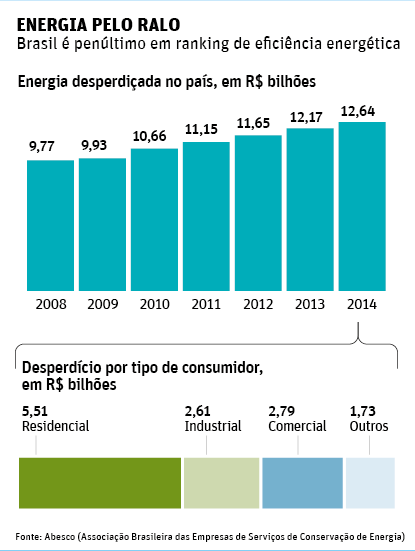
\includegraphics[width=9cm,keepaspectratio]{figuras/desperdicio.jpg}
\caption{\label{fig:desperdicio} Desperdício de Energia no Brasil}
\end{figure}

Dado o cenário desfavorável à geração de energia elétrica e o grande desperdício do consumidor residencial, é imprescindível a tomada de decisões por parte da população. O sistema proposto é composto por dispositivos medidores e de uma aplicação Web que dará ao usuário o conhecimento do perfil de consumo dos seus equipamentos, auxiliando-o a tomar atitudes para diminuição do consumo de energia.

No mercado há várias tecnologias disponíveis para o desenvolvimento do sistema proposto. Para a medição do consumo no equipamento existem sensores, microcontroladores e dispositivos que permitem comunicação sem fio e adaptadores para acesso à internet. Na parte de software, há linguagens de programação gratuitas para o desenvolvimento da aplicação Web, frameworks para agilizar o desenvolvimento e serviços em nuvem para armazenamento e gerenciamento de banco de dados. A existência de tecnologias acessíveis para resolver o problema atual de consumo de energia das residências da região metropolitana de São Paulo motivou o desenvolvimento desse projeto.

\section{Justificativa}
\label{Sec:justificativa}

O sistema proposto atende as necessidades do usuário de várias formas. Através dos gráficos de consumo por equipamento, o usuário poderá perceber que os seus equipamentos em \textit{standby} consomem energia significativa ao longo do tempo. Além disso pode-se detectar possíveis defeitos técnicos nos equipamentos e que, por isso, tendem a consumir mais energia do que deveriam.

Os gráficos do sistema associados a disponibilidade proporcionada pela nuvem, a aplicação Web permite ao usuário monitorar os seus equipamentos a partir de qualquer dispositivo móvel que tenha em mãos com acesso à internet. Com isso, é possível detectar fora da residência aparelhos ligados sem necessidade, por exemplo, ar-condicionado numa sala vazia.

O sistema pode ser utilizado como parte da residência, monitorando 24 horas por dia o consumo dos equipamento, ou pode ser utilizado como um serviço. O usuário contrata o serviço e os dispositivos de medição são instalados em sua residência por um período determinado. Após esse período, são feitas avaliações dos consumos por uma equipe técnica, que poderá recomendar a troca ou a diminuição de consumo de determinados equipamentos apontados pelo sistema.

Tendo em vista as aplicações possíveis para o sistema e os benefícios que o sistema traz para o usuário, o desenvolvimento desse sistema é justificável.

\section{Organização}
\label{Sec:organizacao}

O documento segue o seguinte formato: no capítulo dois são apresentados os conceitos estudados para o desenvolvimento do projeto.

No capítulo três é apresentado o método adotado pelos integrantes do projeto para a realização do projeto do início ao fim.

No capítulo quatro é apresentada a especificação do sistema para o hardware e software.

No capítulo cinco o processo de implementação do projeto é detalhado.

No capítulo seis é detalhado o procedimento de aceitação do sistema através da aplicação de um plano de testes.

No capítulo sete são apontadas algumas considerações finais como aprendizado, dificuldades e resultados atingidos.

No capítulo oito são citadas algumas ideias que poderiam ser aplicadas a trabalhos futuros.
